%!Tex root = bare_conf.tex

% 일반적으로, implementation은 algorithm 뒤에 오는 경우가 많음.
\section{Method}
We implemented two versions of MCTS for Da Vinci code. 
Firstly, we implemented the MCTS algorithm for Da vinci code (\cpu) which is running upon CPU environment.
We used OpenMP to parallelize the algorithm.
Secondly, we implemented the same algorithm which is running upon GPU environment (\gpu).
We used cuda to implement and parallelize the algorithm.

% Both versions are implemented in parallel. 
In the remaining of this section, we describes each version of algorithm in detail. 
As we modified the algorithm due to compuation overhead, we explain the algorithm design considerations compared to the vanilla version of MCTS.

\subsection{Designing Simplified Algorithm}

\begin{figure}
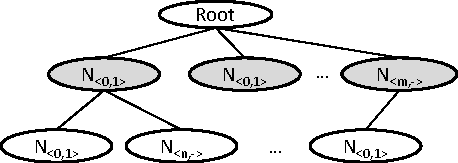
\includegraphics[width=0.95\columnwidth]{figures/base_tree.pdf}
\caption{Tree for Da Vinci Code}
\label{fig:base_tree}
\end{figure}

We designed the tree that each node represents the guessing tile's postion and guessing number~(\cref{fig:base_tree}).
% The \cref{fig:base_tree} shows the overall of MCTS for Da Vinci Code. 
Each node has position and number which are values that a player guesses.
Inherently, depth of tree means the number of guessing until the node.
As players in Da Vinci Code game do not know about other player's tile number, all simulations must be done in black-box manner.
We solve this problem by calculating plausible numbers of opponents tiles.
In each simulation, we randomly picked a set of plausible numbers of the tils, and conducted a simulation according to the numbers.
In this case, the same guessings (e.g., 5 to the leftmost tile) may induce the different results in the different simulation.
Therefore, a node must have information of the set of number to differentiate the results.
We treated this algorithm as a vanilla Da Vinci Code algorithm (\md).

% We implement simplified algorithm to reduce computation and proceed on real time, since original Da Vinci code has a lot of sibling nodes and child nodes which require a huge amount of computation and time limitation. 


We modified three parts of \md~to simplify the problem.
At first, we ignored a set of plausible numbers in view of node.
When we consider a set of plausible numbers, the number of child nodes is exploded.
For example, at the first turn, the root node can have at least 11880 number of chiled nodes.
We compute the number conservatively by considering the case that the opponent have the same colored four tiles.
Though the number is minimum of the number of cases, the number is much higher than 361, the number of go's.
We decided to ignore the set of plausible numbers, and only think of guessing position and guessing number because too many child nodes harm the quality of decision.
By ignoring, we decreased the number

First one is that a player who plays Da Vinci code has two behaviors in each turn, when he/she guesses the tiles. 
Two behaviors are stop and keepping guess.
If the player guesses correctly, play can select stop or keepping guess. 
Therefore, Original Da Vinci code makes depending on the player's choice. 
However, we implemented Da Vinci code that only stop whether the player hits the tile or not. 
Since original Da vinci code has numerous of child node which make the decision tree unbalanced, we decided to implemente simple Da Vinci code which only has stop behavior.
 
\begin{figure}
\begin{subfigure}[b]{0.95\columnwidth}
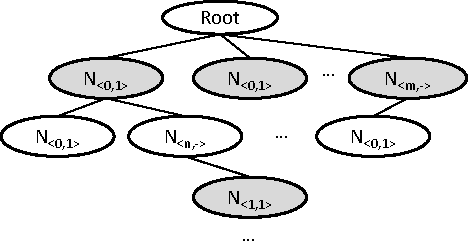
\includegraphics [width=0.95\columnwidth]{figures/sub_compare_expansion_1.pdf}
\caption{MCST with unlimited expansion}
\label{fig:expansion}
\end{subfigure}
\par\bigskip
\begin{subfigure}[b]{0.95\columnwidth}
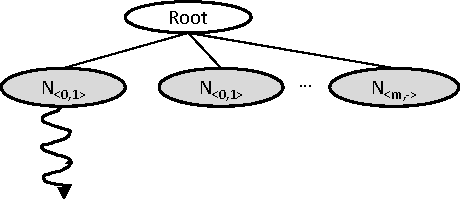
\includegraphics [width=0.95\columnwidth]{figures/sub_compare_expansion_2.pdf}
\caption{MCST with limited expansion}
\label{fig:limited_expansion}
\end{subfigure}
\caption{Comparing vanilla MCTS with simplified MCTS}
\end{figure}

Second one is original MCTS makes expansion to make decision make tree, but we simplified MCTS. 
Since Da Vinci Code has 000000 on each depth, the number of cases makes a number of sibling nodes too hard to compute decision through MCTS. 
In addition, too many cases make wrong decision, because root node has nodes that have similar winning rate. 
Therefore, MCTS which we implemented has limitation of expansion. 
The \cref{fig:expansion} and \cref{fig:limited_expansion}shows the difference bewteen original MCTS and MCTS which we implemented. 
We make one expansion from root and then the remaining turns are proceeded randomly. 
The result of game updates expanded node from root and the MCTS doesn't make other expansion from frist depth. 


\begin{figure}
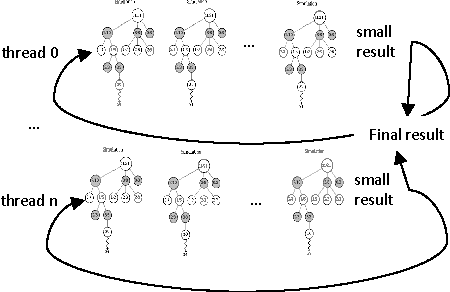
\includegraphics[width=0.95\columnwidth]{figures/implementation.pdf}
\caption{Overall process of creating MCTS}
\label{fig:implementation}
\end{figure}

\subsection{Implementation overview}
To make final MCTS both of CPU and GPU, each thread make small MCTS by simulating a couple of games.
At this time, MCTS is conducted based on current state of own player and an oppenent.
As playing some games within a thread, a simulation makes small MCTS.
Each game in a thread expands the child node from root. 
When the game expands the child node at the frist turn in a thread, the game proceed randomly. 
The result of game rolls out parent node and is updated on the node which is depth one. 
The next game also expands the child node from the root and update the result of game to expanded node (depth one).
Each tread repeats this routin to make small MCTS. 
The threads have small trees which is from simulation and these trees are combined to final MCTS which is used for decision making in Da Vinci code. 
The \cref{fig:implementation} shows the overall process how the MCTS is conducted.
When the player comes to the turn, threads make final MCTS based on current state of the player and the oppenent. 
The player makes the decision based on the final MCTS. 

\subsection{Implementation of \cpu}
MCTS needs many simulated play repeatly to make good decision. 
Parallelism can make MCTS construct good decision tree in a short period due to computating simultaneously. 
MCTS based on CPU is implemented by openMP to utilize parallelism. Each thread computes some turns and derivates a result(win or lose). 
After finish derivation of result, all results from each thread are combined one MCTS.


\subsection{Implementation of \gpu}
As we mentioned, MCTS need parallelism to computation many cases for good decision. 
In GPU version, we use CUDA for paraller computation. 
Each tread computes a couple of turns and derivates a result(win or lose) as same as CPU version. 
After finish derivation of result, the results from each tread are combined final MCTS. 